% Options for packages loaded elsewhere
\PassOptionsToPackage{unicode}{hyperref}
\PassOptionsToPackage{hyphens}{url}
\PassOptionsToPackage{dvipsnames,svgnames,x11names}{xcolor}
%
\documentclass[
  11pt,
]{article}
\usepackage{amsmath,amssymb}
\usepackage{lmodern}
\usepackage{iftex}
\ifPDFTeX
  \usepackage[T1]{fontenc}
  \usepackage[utf8]{inputenc}
  \usepackage{textcomp} % provide euro and other symbols
\else % if luatex or xetex
  \usepackage{unicode-math}
  \defaultfontfeatures{Scale=MatchLowercase}
  \defaultfontfeatures[\rmfamily]{Ligatures=TeX,Scale=1}
\fi
% Use upquote if available, for straight quotes in verbatim environments
\IfFileExists{upquote.sty}{\usepackage{upquote}}{}
\IfFileExists{microtype.sty}{% use microtype if available
  \usepackage[]{microtype}
  \UseMicrotypeSet[protrusion]{basicmath} % disable protrusion for tt fonts
}{}
\makeatletter
\@ifundefined{KOMAClassName}{% if non-KOMA class
  \IfFileExists{parskip.sty}{%
    \usepackage{parskip}
  }{% else
    \setlength{\parindent}{0pt}
    \setlength{\parskip}{6pt plus 2pt minus 1pt}}
}{% if KOMA class
  \KOMAoptions{parskip=half}}
\makeatother
\usepackage{xcolor}
\usepackage[margin=1in]{geometry}
\usepackage{color}
\usepackage{fancyvrb}
\newcommand{\VerbBar}{|}
\newcommand{\VERB}{\Verb[commandchars=\\\{\}]}
\DefineVerbatimEnvironment{Highlighting}{Verbatim}{commandchars=\\\{\}}
% Add ',fontsize=\small' for more characters per line
\usepackage{framed}
\definecolor{shadecolor}{RGB}{248,248,248}
\newenvironment{Shaded}{\begin{snugshade}}{\end{snugshade}}
\newcommand{\AlertTok}[1]{\textcolor[rgb]{0.94,0.16,0.16}{#1}}
\newcommand{\AnnotationTok}[1]{\textcolor[rgb]{0.56,0.35,0.01}{\textbf{\textit{#1}}}}
\newcommand{\AttributeTok}[1]{\textcolor[rgb]{0.77,0.63,0.00}{#1}}
\newcommand{\BaseNTok}[1]{\textcolor[rgb]{0.00,0.00,0.81}{#1}}
\newcommand{\BuiltInTok}[1]{#1}
\newcommand{\CharTok}[1]{\textcolor[rgb]{0.31,0.60,0.02}{#1}}
\newcommand{\CommentTok}[1]{\textcolor[rgb]{0.56,0.35,0.01}{\textit{#1}}}
\newcommand{\CommentVarTok}[1]{\textcolor[rgb]{0.56,0.35,0.01}{\textbf{\textit{#1}}}}
\newcommand{\ConstantTok}[1]{\textcolor[rgb]{0.00,0.00,0.00}{#1}}
\newcommand{\ControlFlowTok}[1]{\textcolor[rgb]{0.13,0.29,0.53}{\textbf{#1}}}
\newcommand{\DataTypeTok}[1]{\textcolor[rgb]{0.13,0.29,0.53}{#1}}
\newcommand{\DecValTok}[1]{\textcolor[rgb]{0.00,0.00,0.81}{#1}}
\newcommand{\DocumentationTok}[1]{\textcolor[rgb]{0.56,0.35,0.01}{\textbf{\textit{#1}}}}
\newcommand{\ErrorTok}[1]{\textcolor[rgb]{0.64,0.00,0.00}{\textbf{#1}}}
\newcommand{\ExtensionTok}[1]{#1}
\newcommand{\FloatTok}[1]{\textcolor[rgb]{0.00,0.00,0.81}{#1}}
\newcommand{\FunctionTok}[1]{\textcolor[rgb]{0.00,0.00,0.00}{#1}}
\newcommand{\ImportTok}[1]{#1}
\newcommand{\InformationTok}[1]{\textcolor[rgb]{0.56,0.35,0.01}{\textbf{\textit{#1}}}}
\newcommand{\KeywordTok}[1]{\textcolor[rgb]{0.13,0.29,0.53}{\textbf{#1}}}
\newcommand{\NormalTok}[1]{#1}
\newcommand{\OperatorTok}[1]{\textcolor[rgb]{0.81,0.36,0.00}{\textbf{#1}}}
\newcommand{\OtherTok}[1]{\textcolor[rgb]{0.56,0.35,0.01}{#1}}
\newcommand{\PreprocessorTok}[1]{\textcolor[rgb]{0.56,0.35,0.01}{\textit{#1}}}
\newcommand{\RegionMarkerTok}[1]{#1}
\newcommand{\SpecialCharTok}[1]{\textcolor[rgb]{0.00,0.00,0.00}{#1}}
\newcommand{\SpecialStringTok}[1]{\textcolor[rgb]{0.31,0.60,0.02}{#1}}
\newcommand{\StringTok}[1]{\textcolor[rgb]{0.31,0.60,0.02}{#1}}
\newcommand{\VariableTok}[1]{\textcolor[rgb]{0.00,0.00,0.00}{#1}}
\newcommand{\VerbatimStringTok}[1]{\textcolor[rgb]{0.31,0.60,0.02}{#1}}
\newcommand{\WarningTok}[1]{\textcolor[rgb]{0.56,0.35,0.01}{\textbf{\textit{#1}}}}
\usepackage{longtable,booktabs,array}
\usepackage{calc} % for calculating minipage widths
% Correct order of tables after \paragraph or \subparagraph
\usepackage{etoolbox}
\makeatletter
\patchcmd\longtable{\par}{\if@noskipsec\mbox{}\fi\par}{}{}
\makeatother
% Allow footnotes in longtable head/foot
\IfFileExists{footnotehyper.sty}{\usepackage{footnotehyper}}{\usepackage{footnote}}
\makesavenoteenv{longtable}
\usepackage{graphicx}
\makeatletter
\def\maxwidth{\ifdim\Gin@nat@width>\linewidth\linewidth\else\Gin@nat@width\fi}
\def\maxheight{\ifdim\Gin@nat@height>\textheight\textheight\else\Gin@nat@height\fi}
\makeatother
% Scale images if necessary, so that they will not overflow the page
% margins by default, and it is still possible to overwrite the defaults
% using explicit options in \includegraphics[width, height, ...]{}
\setkeys{Gin}{width=\maxwidth,height=\maxheight,keepaspectratio}
% Set default figure placement to htbp
\makeatletter
\def\fps@figure{htbp}
\makeatother
\setlength{\emergencystretch}{3em} % prevent overfull lines
\providecommand{\tightlist}{%
  \setlength{\itemsep}{0pt}\setlength{\parskip}{0pt}}
\setcounter{secnumdepth}{-\maxdimen} % remove section numbering
\usepackage{amsmath,amsthm,amssymb}
\newcommand{\tp}{^\intercal}
\DeclareMathOperator{\E}{\mathbb{E}}
\DeclareMathOperator{\cov}{\mathbb{C}\text{ov}}
\DeclareMathOperator{\var}{\mathbb{V}\text{ar}}
\DeclareMathOperator{\I}{\mathbbm{1}}
\renewcommand{\vec}[1]{\bm{\mathbf #1}}
\usepackage{booktabs}
\usepackage{longtable}
\usepackage{array}
\usepackage{multirow}
\usepackage{wrapfig}
\usepackage{float}
\usepackage{colortbl}
\usepackage{pdflscape}
\usepackage{tabu}
\usepackage{threeparttable}
\usepackage{threeparttablex}
\usepackage[normalem]{ulem}
\usepackage{makecell}
\usepackage{xcolor}
\ifLuaTeX
  \usepackage{selnolig}  % disable illegal ligatures
\fi
\IfFileExists{bookmark.sty}{\usepackage{bookmark}}{\usepackage{hyperref}}
\IfFileExists{xurl.sty}{\usepackage{xurl}}{} % add URL line breaks if available
\urlstyle{same} % disable monospaced font for URLs
\hypersetup{
  pdftitle={PSTAT 220A Section 01},
  pdfauthor={Jaxon Stuhr},
  colorlinks=true,
  linkcolor={Maroon},
  filecolor={Maroon},
  citecolor={Blue},
  urlcolor={blue},
  pdfcreator={LaTeX via pandoc}}

\title{PSTAT 220A Section 01}
\author{Jaxon Stuhr}
\date{September 27, 2022}

\begin{document}
\maketitle

\textbf{Note:} Today's material is from tutorials by
\href{https://ourcodingclub.github.io/tutorials/rmarkdown/}{Coding Club}
and \href{https://rmarkdown.rstudio.com/index.html}{R Studio}.

\hypertarget{r-markdown}{%
\subsection{R Markdown}\label{r-markdown}}

R Markdown is a file format for writing reproducible, dynamic reports
with R. Use it to embed R code and results into slideshows, pdfs, html
documents, word files and more. A \texttt{.Rmd} file is a simple plain
text file with three types of content: \texttt{YAML} metadata, text and
code chunks, like the document below.

\begin{figure}
\begin{center}
#\includegraphics[width=300pt]{RMarkdown.png}
\end{center}
\end{figure}

\textbf{\texttt{YAML} Header}: at the top of any RMarkdown script is a
\texttt{YAML} header section. By default this includes a title, author,
date and the file type you want to output to. Many other options are
available for different functions and formatting, see
\href{https://bookdown.org/yihui/rmarkdown/html-document.html}{here} for
\texttt{.html} options and
\href{https://bookdown.org/yihui/rmarkdown/pdf-document.html}{here} for
\texttt{.pdf} options. Rules in the header section will alter the whole
document.

\textbf{Code Chunks}: below the \texttt{YAML} header is the space where
you will write your code, accompanying explanation and any outputs.
Codes included in your \texttt{.Rmd} document should be enclosed by
chunk delimiters. When you render your \texttt{.Rmd} file, R Markdown
will run each code chunk and embed the results beneath the code chunk in
your final report.

You can also customize chunk output with
\href{https://yihui.org/knitr/options/}{knitr options}. And arguments
are set in the \texttt{\{ \}} of a chunk header. See
\href{https://rstudio.com/wp-content/uploads/2015/03/rmarkdown-reference.pdf?_ga=2.34482913.1386655696.1601928126-343717157.1601928126}{R
Markdown Reference Guide} for a complete list of knitr chunk options.
Moreover, to set global options that apply to every chunk in your file,
call \texttt{knitr::opts\_chunk\$set} in a code chunk. \texttt{Knitr}
will treat each option that you pass to \texttt{knitr::opts\_chunk\$set}
as a global default that can be overwritten in individual chunk headers.

\hypertarget{formatting-text}{%
\subsection{Formatting Text}\label{formatting-text}}

\hypertarget{basic-formatting}{%
\subsubsection{Basic Formatting}\label{basic-formatting}}

I only list some syntax here. See
\href{https://rmarkdown.rstudio.com/lesson-15.html}{R Markdown
Cheatsheets} for more syntax.

\begin{itemize}
\item
  \textbf{Paragraph Breaks}: To insert a break between paragraphs,
  include a single completely blank line. To force a line break, put two
  blank spaces at the end of a line.
\item
  \textbf{Headers}: The character \texttt{\#} at the beginning of a line
  means that the rest of the line is interpreted as a section header.
  The number of \texttt{\#}'s at the beginning of the line indicates
  whether it is treated as a section, sub-section, sub-sub-section, etc.
  of the document.
\item
  \textbf{Italics and Boldface}: Text to be \emph{italicized} goes
  inside a single set of underscores or asterisks. Text to be
  \textbf{boldfaced} goes inside a double set of underscores or
  asterisks.
\end{itemize}

\hypertarget{inline-code}{%
\subsubsection{Inline Code}\label{inline-code}}

Code output can also be seamlessly incorporated into the text, using
\textbf{inline code}. This is code not set off on a line by itself, but
beginning with \texttt{$\grave{\ }$r} and ending with
\texttt{$\grave{\ }$}. Using inline code is how this document knows that
\(1+2+\cdots+100\) equals to 5050.

\hypertarget{mathematical-formula}{%
\subsubsection{Mathematical Formula}\label{mathematical-formula}}

R Markdown gives you the syntax to render complex mathematical formulas
and derivations, and have them displayed very nicely. The syntax is same
as \LaTeX. And like code, the math can either be inline or set off.

Inline mathematical formula is marked off with a pair of dollar signs
(\texttt{\$}), such as \(\bar{X}=\frac{1}{n}\sum_{j=1}^nX_j\).
Mathematical displays are marked off with \texttt{$\backslash$[} and
\texttt{$\backslash$]}, as in

\begin{verbatim}
\[
\bar{X}=\frac{1}{n}\sum_{j=1}^nX_j
\]
\end{verbatim}

\[
\bar{X}=\frac{1}{n}\sum_{j=1}^nX_j.
\]

You can also use environments, such as \texttt{align},
\texttt{eqnarray}, and etc. from \LaTeX. See section 3.10 from
\href{https://mirror.las.iastate.edu/tex-archive/info/lshort/english/lshort.pdf}{\emph{The
Not So Short Introduction to \LaTeXe}} for list of mathematical symbols.

\hypertarget{inserting-figures}{%
\subsection{Inserting Figures}\label{inserting-figures}}

Inserting a graph generated by \texttt{R} into RMarkdown is relatively
easy. By default, RMarkdown will place graphs by maximizing their
height, while keeping them within the margins of the page and
maintaining aspect ratio. And to manually set the figure dimensions, you
can insert an instruction into the curly braces:

\begin{Shaded}
\begin{Highlighting}[]
\FunctionTok{library}\NormalTok{(ISLR) }
\FunctionTok{data}\NormalTok{(}\StringTok{"Wage"}\NormalTok{) }
\FunctionTok{boxplot}\NormalTok{(wage}\SpecialCharTok{\textasciitilde{}}\FunctionTok{unclass}\NormalTok{(education),}\AttributeTok{data=}\NormalTok{Wage,}\AttributeTok{pch=}\DecValTok{19}\NormalTok{,}\AttributeTok{cex=}\FloatTok{0.5}\NormalTok{,}
        \AttributeTok{col=}\FunctionTok{c}\NormalTok{(}\StringTok{"\#5fa5d6"}\NormalTok{,}\StringTok{"\#08966c"}\NormalTok{,}\StringTok{"\#d2dd4e"}\NormalTok{,}\StringTok{"\#1d70b0"}\NormalTok{,}\StringTok{"\#cc6320"}\NormalTok{),}
        \AttributeTok{xlab=}\StringTok{"Education Level"}\NormalTok{,}\AttributeTok{ylab=}\StringTok{"Wage"}\NormalTok{)}
\end{Highlighting}
\end{Shaded}

\begin{center}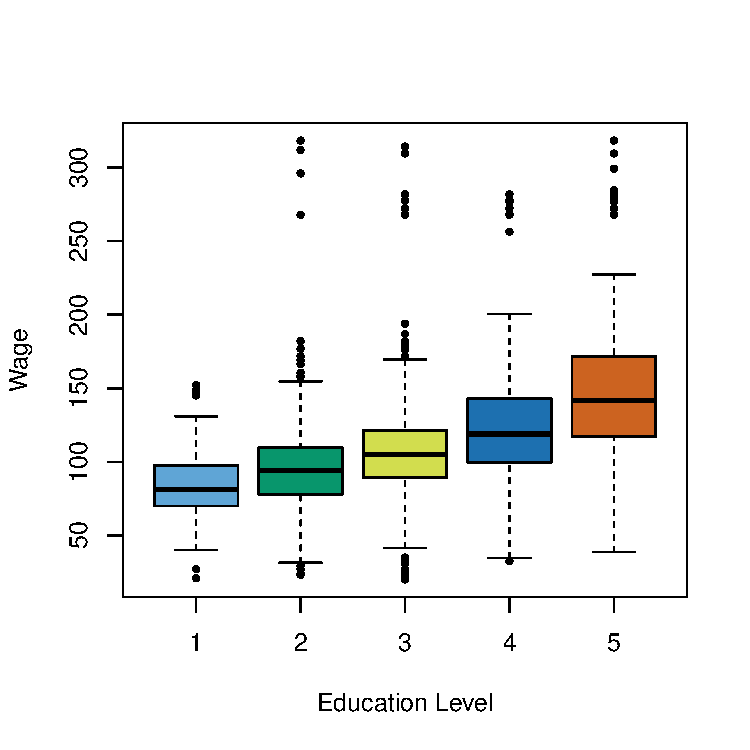
\includegraphics{lab_1_files/figure-latex/unnamed-chunk-2-1} \end{center}

You can also insert a local image by the following syntax:

\begin{verbatim}
 ![](path/to/smallorb.png)
\end{verbatim}

However, it is not easy to adjust the location and parameters of a
figure by the above code. I would recommend you to use the picture
environment from \LaTeX.

\hypertarget{inserting-tables}{%
\subsection{Inserting Tables}\label{inserting-tables}}

Tables are important in statistical reports. There are several ways to
insert tables in your \texttt{.Rmd} files. And we first create the
following data frame, and then use it for illustration.

\begin{Shaded}
\begin{Highlighting}[]
\NormalTok{Plant }\OtherTok{\textless{}{-}} \FunctionTok{c}\NormalTok{(}\StringTok{"A"}\NormalTok{, }\StringTok{"B"}\NormalTok{, }\StringTok{"C"}\NormalTok{)}
\NormalTok{Temp. }\OtherTok{\textless{}{-}} \FunctionTok{c}\NormalTok{(}\DecValTok{20}\NormalTok{, }\DecValTok{20}\NormalTok{, }\DecValTok{20}\NormalTok{)}
\NormalTok{Growth }\OtherTok{\textless{}{-}} \FunctionTok{c}\NormalTok{(}\FloatTok{0.65}\NormalTok{, }\FloatTok{0.95}\NormalTok{, }\FloatTok{0.15}\NormalTok{)}
\NormalTok{da }\OtherTok{\textless{}{-}} \FunctionTok{data.frame}\NormalTok{(Plant, Temp., Growth)}
\end{Highlighting}
\end{Shaded}

You can directly print the content of a data frame with the following
syntax.

\begin{Shaded}
\begin{Highlighting}[]
\NormalTok{da}
\end{Highlighting}
\end{Shaded}

\begin{verbatim}
##   Plant Temp. Growth
## 1     A    20   0.65
## 2     B    20   0.95
## 3     C    20   0.15
\end{verbatim}

However, this table looks a bit messy.

\hypertarget{function-in-package}{%
\subsubsection{\texorpdfstring{\texttt{kable( )} function in
\texttt{knitr}
package}{ function in  package}}\label{function-in-package}}

The simplest table formatting function is \texttt{kable( )} function in
\texttt{knitr} package. The first argument tells \texttt{kable} to make
a table out of the target data frame and that numbers should have at
most two digits.

\begin{Shaded}
\begin{Highlighting}[]
\FunctionTok{kable}\NormalTok{(da, }\AttributeTok{digits =} \DecValTok{2}\NormalTok{)}
\end{Highlighting}
\end{Shaded}

\begin{tabular}{l|r|r}
\hline
Plant & Temp. & Growth\\
\hline
A & 20 & 0.65\\
\hline
B & 20 & 0.95\\
\hline
C & 20 & 0.15\\
\hline
\end{tabular}

See
\href{https://haozhu233.github.io/kableExtra/awesome_table_in_pdf.pdf}{\emph{Create
Awesome \LaTeX Table with \texttt{knitr::kable} and
\texttt{kableExtra}}} for more details and examples.

\hypertarget{manually-creating-tables-using-markdown-syntax}{%
\subsubsection{Manually creating tables using markdown
syntax}\label{manually-creating-tables-using-markdown-syntax}}

You can also manually create small tables using markdown syntax. For
example:

\begin{verbatim}
| Plant | Temp. | Growth |
|:------|:-----:|-------:|
| A     | 20    | 0.65   |
| B     | 20    | 0.95   |
| C     | 20    | 0.15   |
\end{verbatim}

will create something that looks like this:

\begin{longtable}[]{@{}lcr@{}}
\toprule()
Plant & Temp. & Growth \\
\midrule()
\endhead
A & 20 & 0.65 \\
B & 20 & 0.95 \\
C & 20 & 0.15 \\
\bottomrule()
\end{longtable}

The \texttt{:-----:} tells markdown that the line above should be
treated as a header and the lines below should be treated as the body of
the table. Text alignment of the columns is set by the position of
\texttt{:}.

\emph{\textbf{Get your hand dirty, and try to write your homework with R
Markdown!}}

\end{document}
